\documentclass{report}
\usepackage{tikz}
\usepackage{subcaption}

\begin{document}
\begin{figure}
  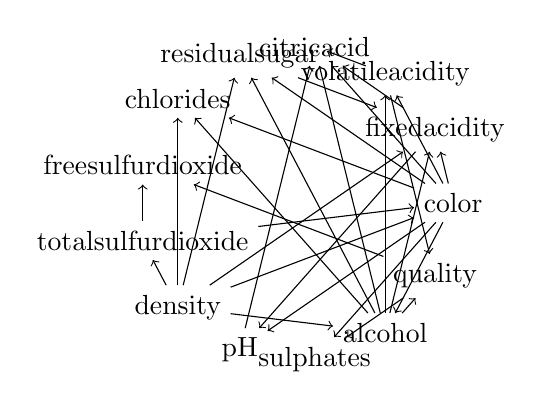
\begin{tikzpicture}
      \draw
        (0.0:2) node (color){color}
        (27.692:2) node (fixedacidity){fixedacidity}
        (55.385:2) node (volatileacidity){volatileacidity}
        (83.077:2) node (citricacid){citricacid}
        (110.769:2) node (residualsugar){residualsugar}
        (138.462:2) node (chlorides){chlorides}
        (166.154:2) node (freesulfurdioxide){freesulfurdioxide}
        (193.846:2) node (totalsulfurdioxide){totalsulfurdioxide}
        (221.538:2) node (density){density}
        (249.231:2) node (pH){pH}
        (276.923:2) node (sulphates){sulphates}
        (304.615:2) node (alcohol){alcohol}
        (332.308:2) node (quality){quality};
      \begin{scope}[->]
        \draw (color) to (fixedacidity);
        \draw (color) to (volatileacidity);
        \draw (color) to (citricacid);
        \draw (color) to (residualsugar);
        \draw (color) to (chlorides);
        \draw (color) to (pH);
        \draw (color) to (sulphates);
        \draw (color) to (alcohol);
        \draw (fixedacidity) to (citricacid);
        \draw (fixedacidity) to (pH);
        \draw (volatileacidity) to (quality);
        \draw (citricacid) to (volatileacidity);
        \draw (residualsugar) to (fixedacidity);
        \draw (totalsulfurdioxide) to (color);
        \draw (totalsulfurdioxide) to (freesulfurdioxide);
        \draw (density) to (color);
        \draw (density) to (fixedacidity);
        \draw (density) to (residualsugar);
        \draw (density) to (chlorides);
        \draw (density) to (totalsulfurdioxide);
        \draw (density) to (alcohol);
        \draw (pH) to (citricacid);
        \draw (alcohol) to (fixedacidity);
        \draw (alcohol) to (volatileacidity);
        \draw (alcohol) to (citricacid);
        \draw (alcohol) to (residualsugar);
        \draw (alcohol) to (chlorides);
        \draw (alcohol) to (quality);
        \draw (quality) to (freesulfurdioxide);
        \draw (quality) to (sulphates);
      \end{scope}
    \end{tikzpicture}
  \caption{medium}
\end{figure}
\end{document}